\documentclass[a4paper]{article}
\usepackage[pdftex]{hyperref}
\usepackage[latin1]{inputenc}
\usepackage[english]{babel}
\usepackage{a4wide}
\usepackage{amsmath}
\usepackage{amssymb}
\usepackage{algorithmic}
\usepackage{algorithm}
\usepackage{graphicx}
\usepackage{ifthen}
\usepackage{listings}
% move the asterisk at the right position
\lstset{basicstyle=\ttfamily,tabsize=4,literate={*}{${}^*{}$}1}
%\lstset{language=C,basicstyle=\ttfamily}
\usepackage{moreverb}
\usepackage{palatino}
\usepackage{multicol}
\usepackage{tabularx}
\usepackage{comment}
\usepackage{verbatim}
\usepackage{color}
\usepackage{tikz}
\usetikzlibrary{arrows,shapes.gates.logic.US,shapes.gates.logic.IEC,calc}
%% pdflatex?
\newif\ifpdf
\ifx\pdfoutput\undefined
\pdffalse % we are not running PDFLaTeX
\else
\pdfoutput=1 % we are running PDFLaTeX
\pdftrue
\fi

\ifpdf
\DeclareGraphicsExtensions{.pdf, .jpg}
\else
\DeclareGraphicsExtensions{.eps, .jpg}
\fi

\parindent=0cm
\parskip=0cm

\setlength{\columnseprule}{0.4pt}
\addtolength{\columnsep}{2pt}

\addtolength{\textheight}{5.5cm}
\addtolength{\topmargin}{-26mm}
\pagestyle{empty}

%%
%% Sheet setup
%% 
\newcommand{\coursename}{Computer Networks}

 
\newcommand{\sheettitle}{Homework}
\newcommand{\mytitle}{}
\newcommand{\mytoday}{\textcolor{blue}{March 15th}, 2020}

% Current Assignment number
\newcounter{assignmentno}
\setcounter{assignmentno}{2}

% Current Problem number, should always start at 1
\newcounter{problemno}
\setcounter{problemno}{1}

%%
%% problem and bonus environment
%%
\newcounter{probcalc}
\newcommand{\problem}[2]{
  \pagebreak[2]
  \setcounter{probcalc}{#2}
  ~\\
  {\large \textbf{Problem \textcolor{blue}{\arabic{assignmentno}}.\textcolor{blue}{\arabic{problemno}}} \hspace{0.2cm}\textit{#1}} \refstepcounter{problemno}\vspace{2pt}\\}

\newcommand{\bonus}[2]{
  \pagebreak[2]
  \setcounter{probcalc}{#2}
  ~\\
  {\large \textbf{Bonus Problem \textcolor{blue}{\arabic{assignmentno}}.\textcolor{blue}{\arabic{problemno}}} \hspace{0.2cm}\textit{#1}} \refstepcounter{problemno}\vspace{2pt}\\}

%% some counters  
\newcommand{\assignment}{\arabic{assignmentno}}

%% solution  
\newcommand{\solution}{\pagebreak[2]{\bf Solution:}\\}

%% Hyperref Setup
\hypersetup{pdftitle={Homework \assignment},
  pdfsubject={\coursename},
  pdfauthor={},
  pdfcreator={},
  pdfkeywords={Computer Architecture and Programming Languages},
  %  pdfpagemode={FullScreen},
  %colorlinks=true,
  %bookmarks=true,
  %hyperindex=true,
  bookmarksopen=false,
  bookmarksnumbered=true,
  breaklinks=true,
  %urlcolor=darkblue
  urlbordercolor={0 0 0.7}
}

\begin{document}
\coursename \hfill 
Jacobs University Bremen \hfill \mytoday\\
\textcolor{blue}{Arsenij Percov}\hfill
\vspace*{0.3cm}\\
\begin{center}
{\Large \sheettitle{} \textcolor{blue}{\assignment}\\}
\end{center}

\problem{}{0}
\solution
a)\\
i)\\Root bridge is the one with the lowest priority:in our case every bridge has same priority. It is a tie, and we resolve a tie by selecting a bridge with the lowest ID. Therefore, the bridge B1 is the root.\\
We choose (In this case manually) shortest path from each bridge to the root bridge, and mark root port.
\\
\begin{tabular}{|c|c|c|}
\hline
Bridge & Shortest Path & Root Port\\\hline
B2 & B2 $\rightarrow$ B1 & P2.2\\\hline
B3 & B3 $\rightarrow$ B2  $\rightarrow$ B1 & P3.2\\\hline
B4 & B4 $\rightarrow$ B1 & P4.2\\\hline
B5 & B5 $\rightarrow$ B3 $\rightarrow$ B2 $\rightarrow$ B1 & P5.1\\\hline
B6 & B6 $\rightarrow$ B2 $\rightarrow$ B1 & P6.1\\\hline
B7 & B7 $\rightarrow$ B4 $\rightarrow$ B1 & P7.1\\\hline
B8 & B8 $\rightarrow$ B1 & P8.2\\\hline

\end{tabular}\\

Next, we can circle with black color the root ports, and we indicate root.\\
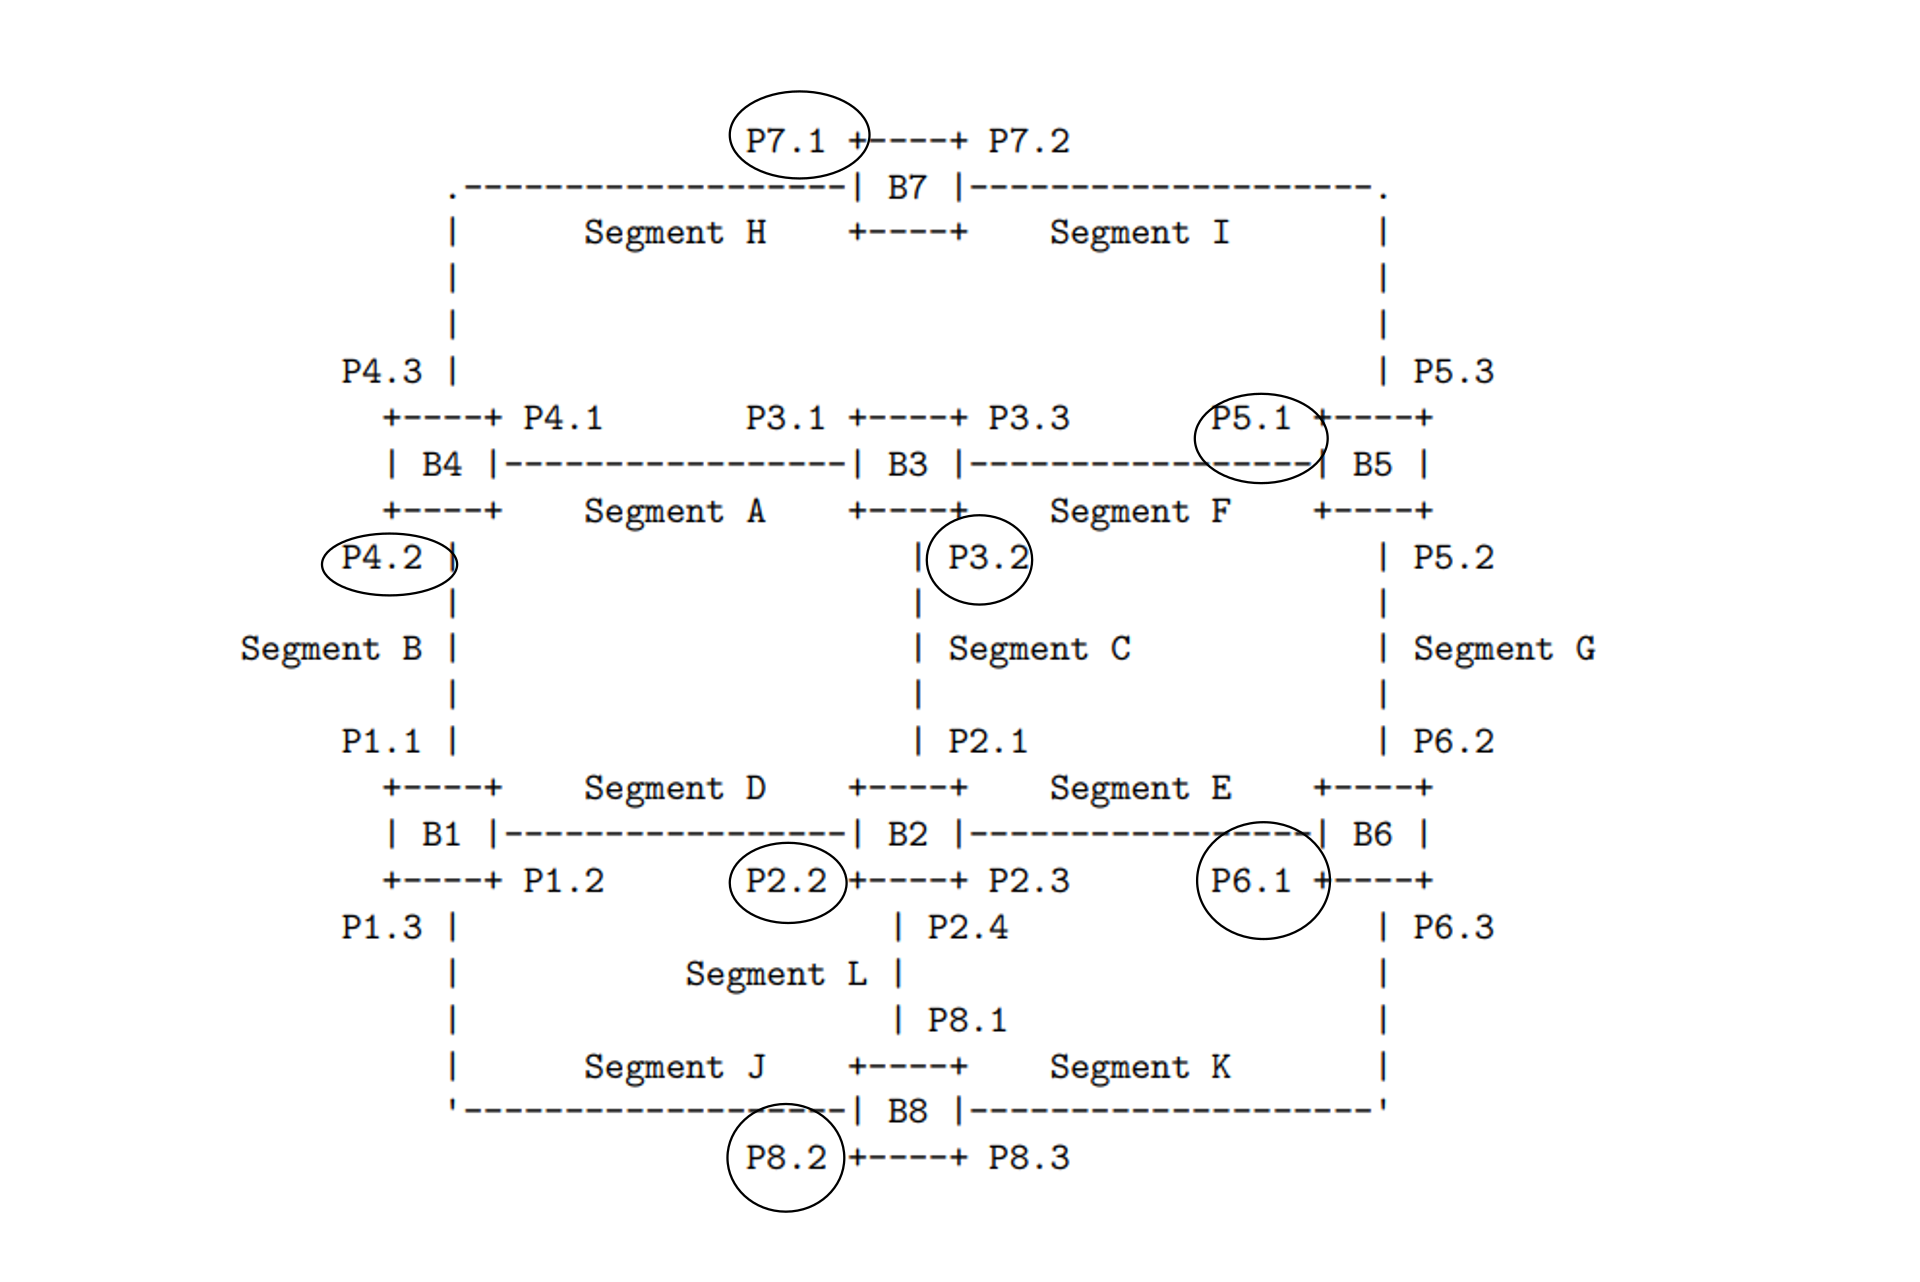
\includegraphics[scale=0.2]{aww-board.png}\\
ii)
Next we locate designated ports:
First, we selected every port that has root port on the other end of segment.(designated ports in green).\\
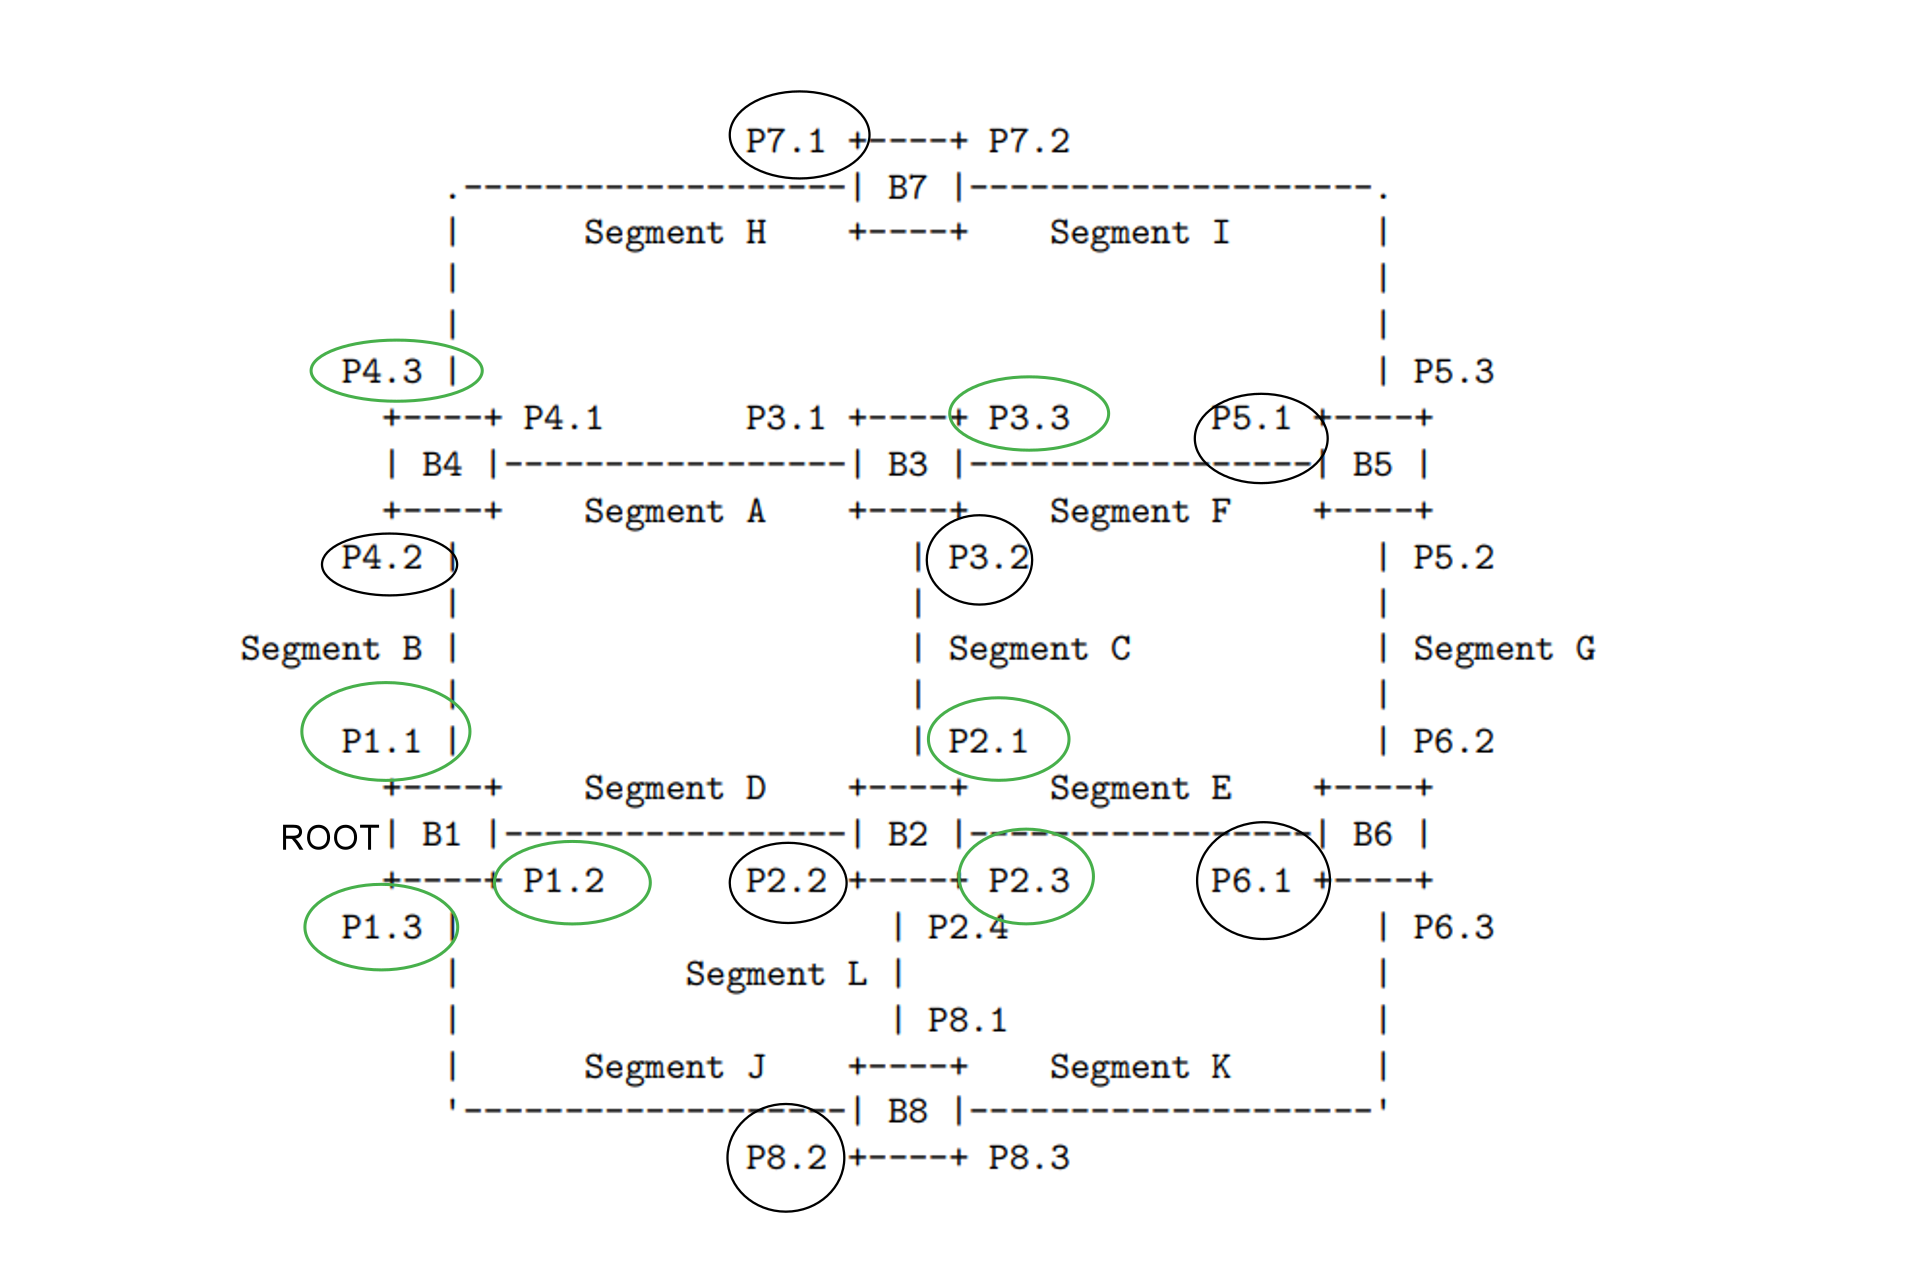
\includegraphics[scale=0.2]{des-port.png}\\
\\
Next we look on all the unused segments, and select one of the ports on them to be designated port, the other part in next bullet point of answer will be selected as a blocked one.\\
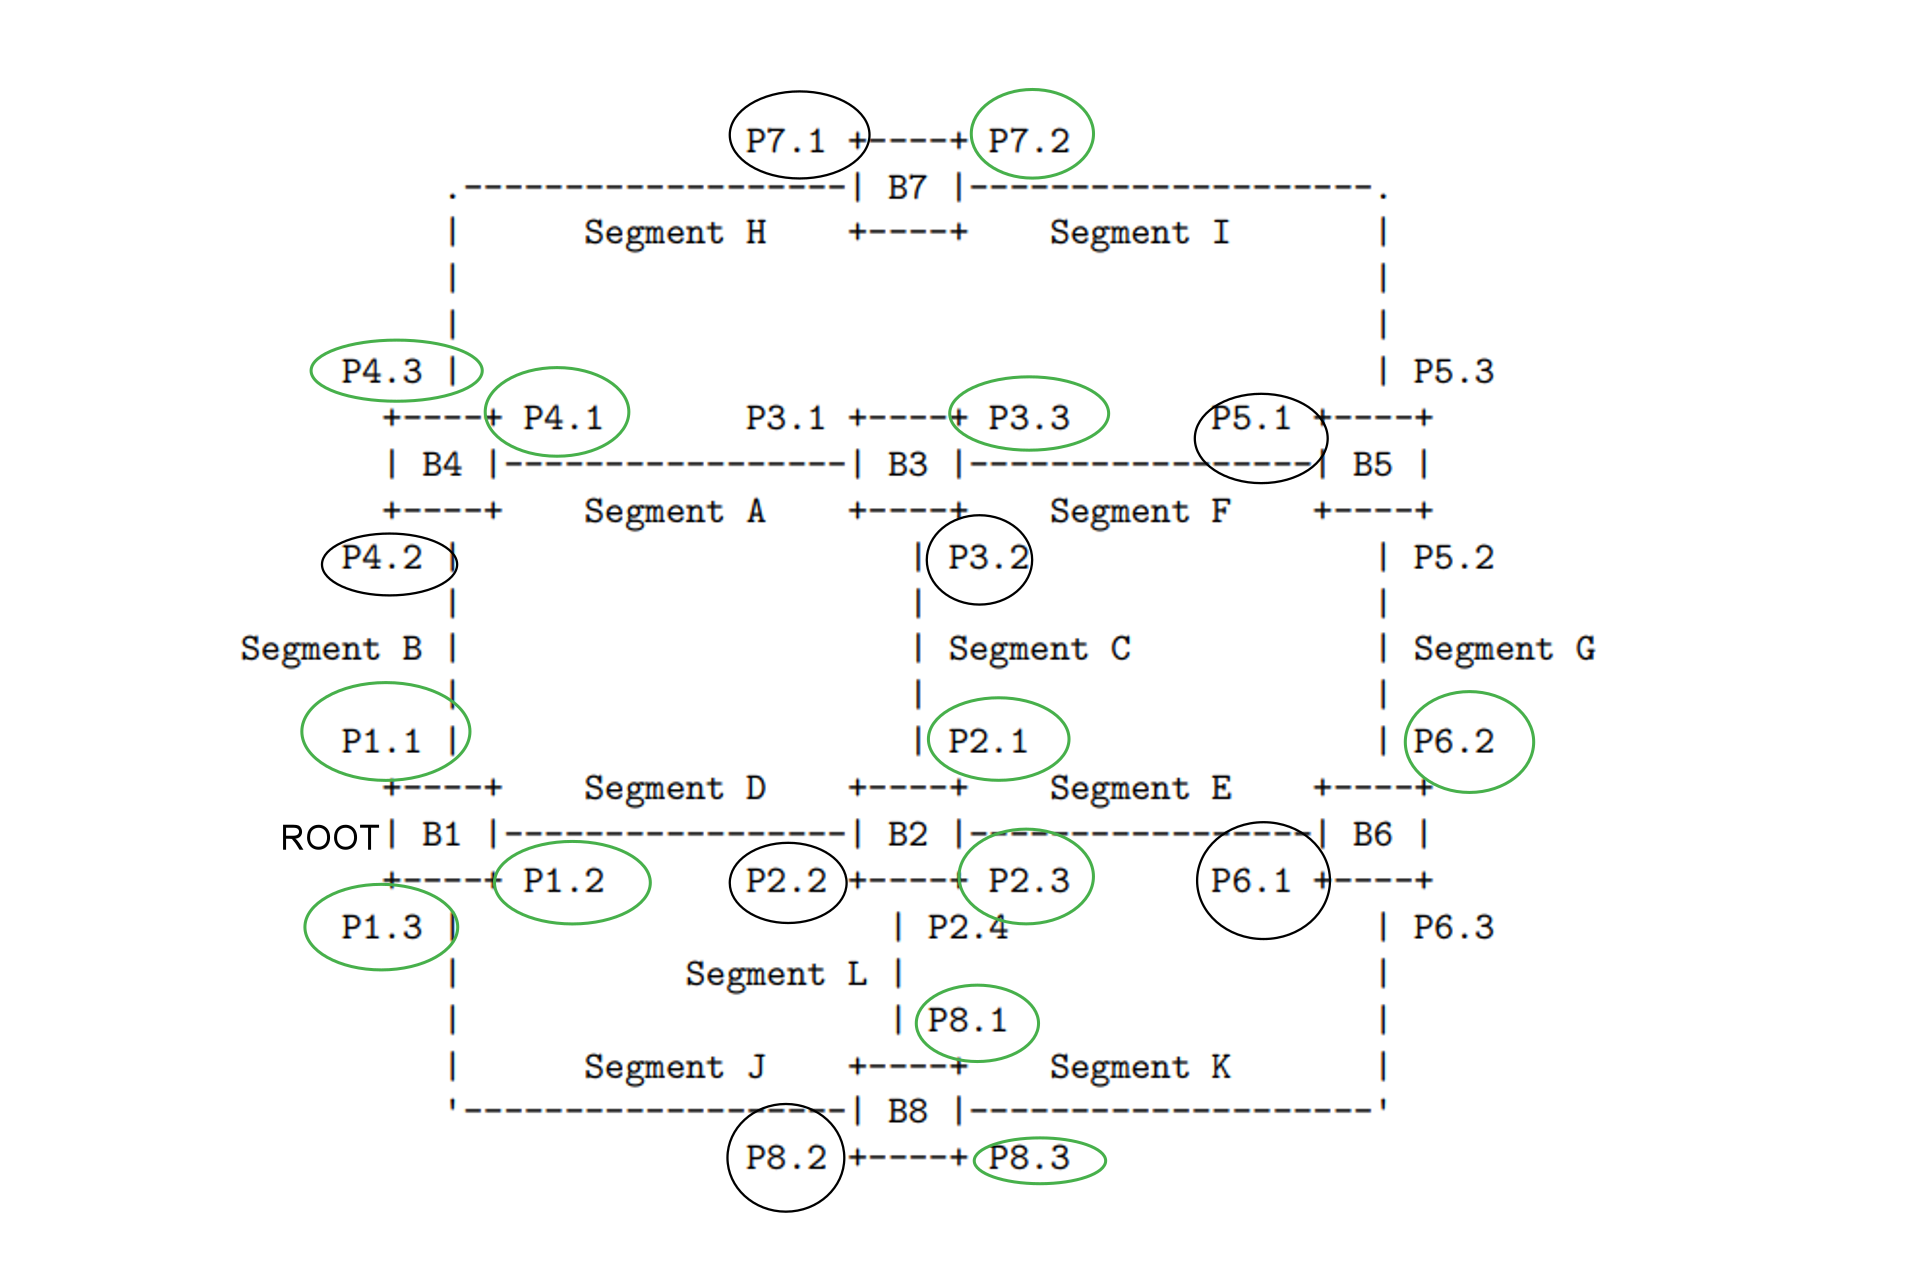
\includegraphics[scale=0.2]{aww-board-2.png}
\\\\
iii)All the other ports are blocked ports(circled in red).\\
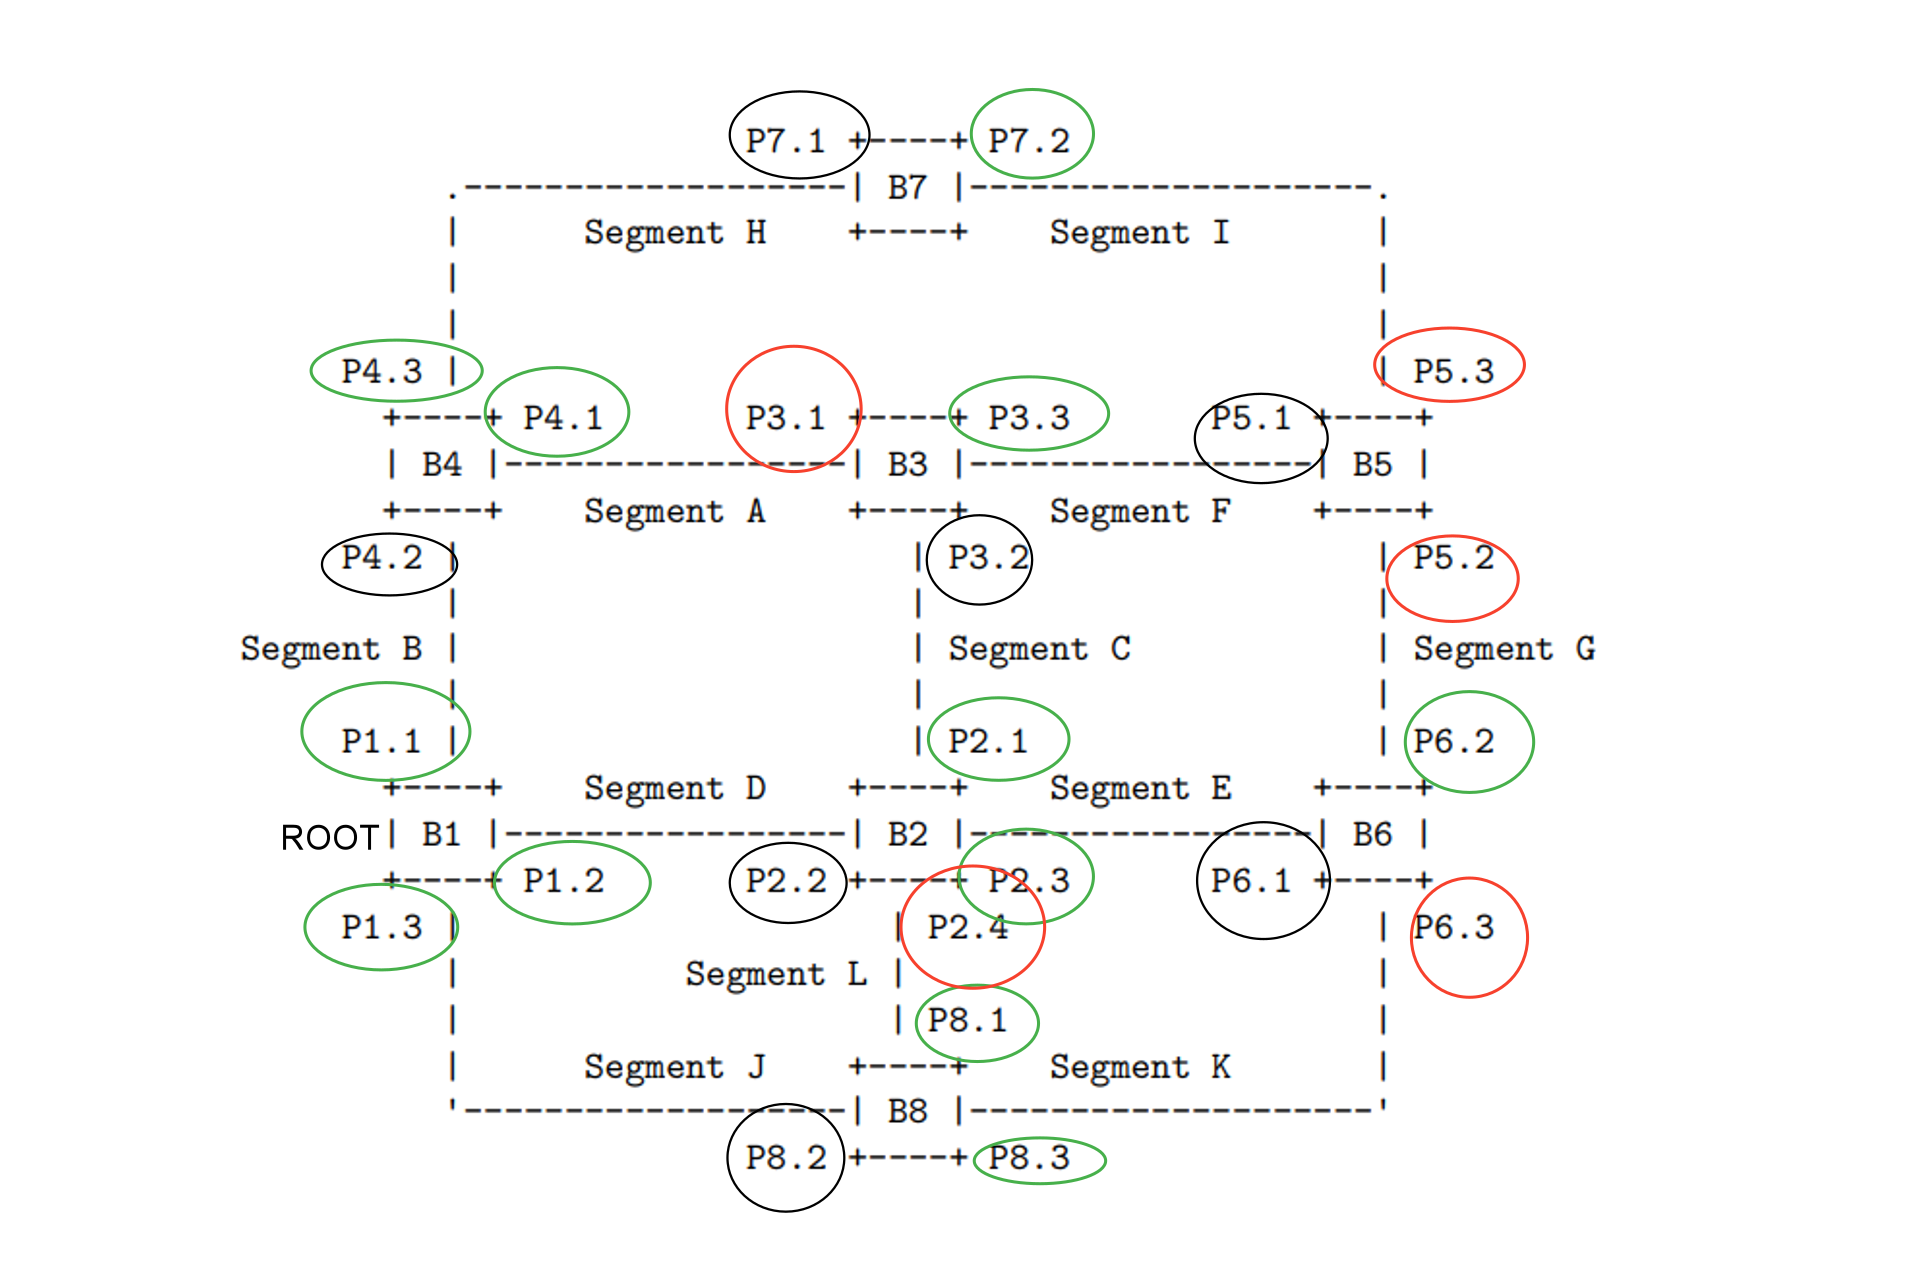
\includegraphics[scale=0.2]{aww-board-3.png}\\
\\
\\
b)
\\
i)\\
First root is selected, we have same case as last time with priority, so we choose lowest id, which is in this case B2, as the root bridge.\\
We choose (In this case manually) shortest path from each bridge to the root bridge, and mark root port.
\\
\begin{tabular}{|c|c|c|}
\hline
Bridge & Shortest Path & Root Port\\\hline
B3 & B3 $\rightarrow$ B2 & P3.2\\\hline
B4 & B4 $\rightarrow$ B3 $\rightarrow$ B2 & P4.1\\\hline
B5 & B5 $\rightarrow$ B3 $\rightarrow$ B2 & P5.1\\\hline
B6 & B6 $\rightarrow$ B2 & P6.1\\\hline
B7 & B7 $\rightarrow$ B4 $\rightarrow$ B3 $\rightarrow$ B2 & P7.1\\\hline
B8 & B8 $\rightarrow$ B2 & P8.1\\\hline

\end{tabular}\\

Next, we can circle with black color the root ports, and we indicate root.\\
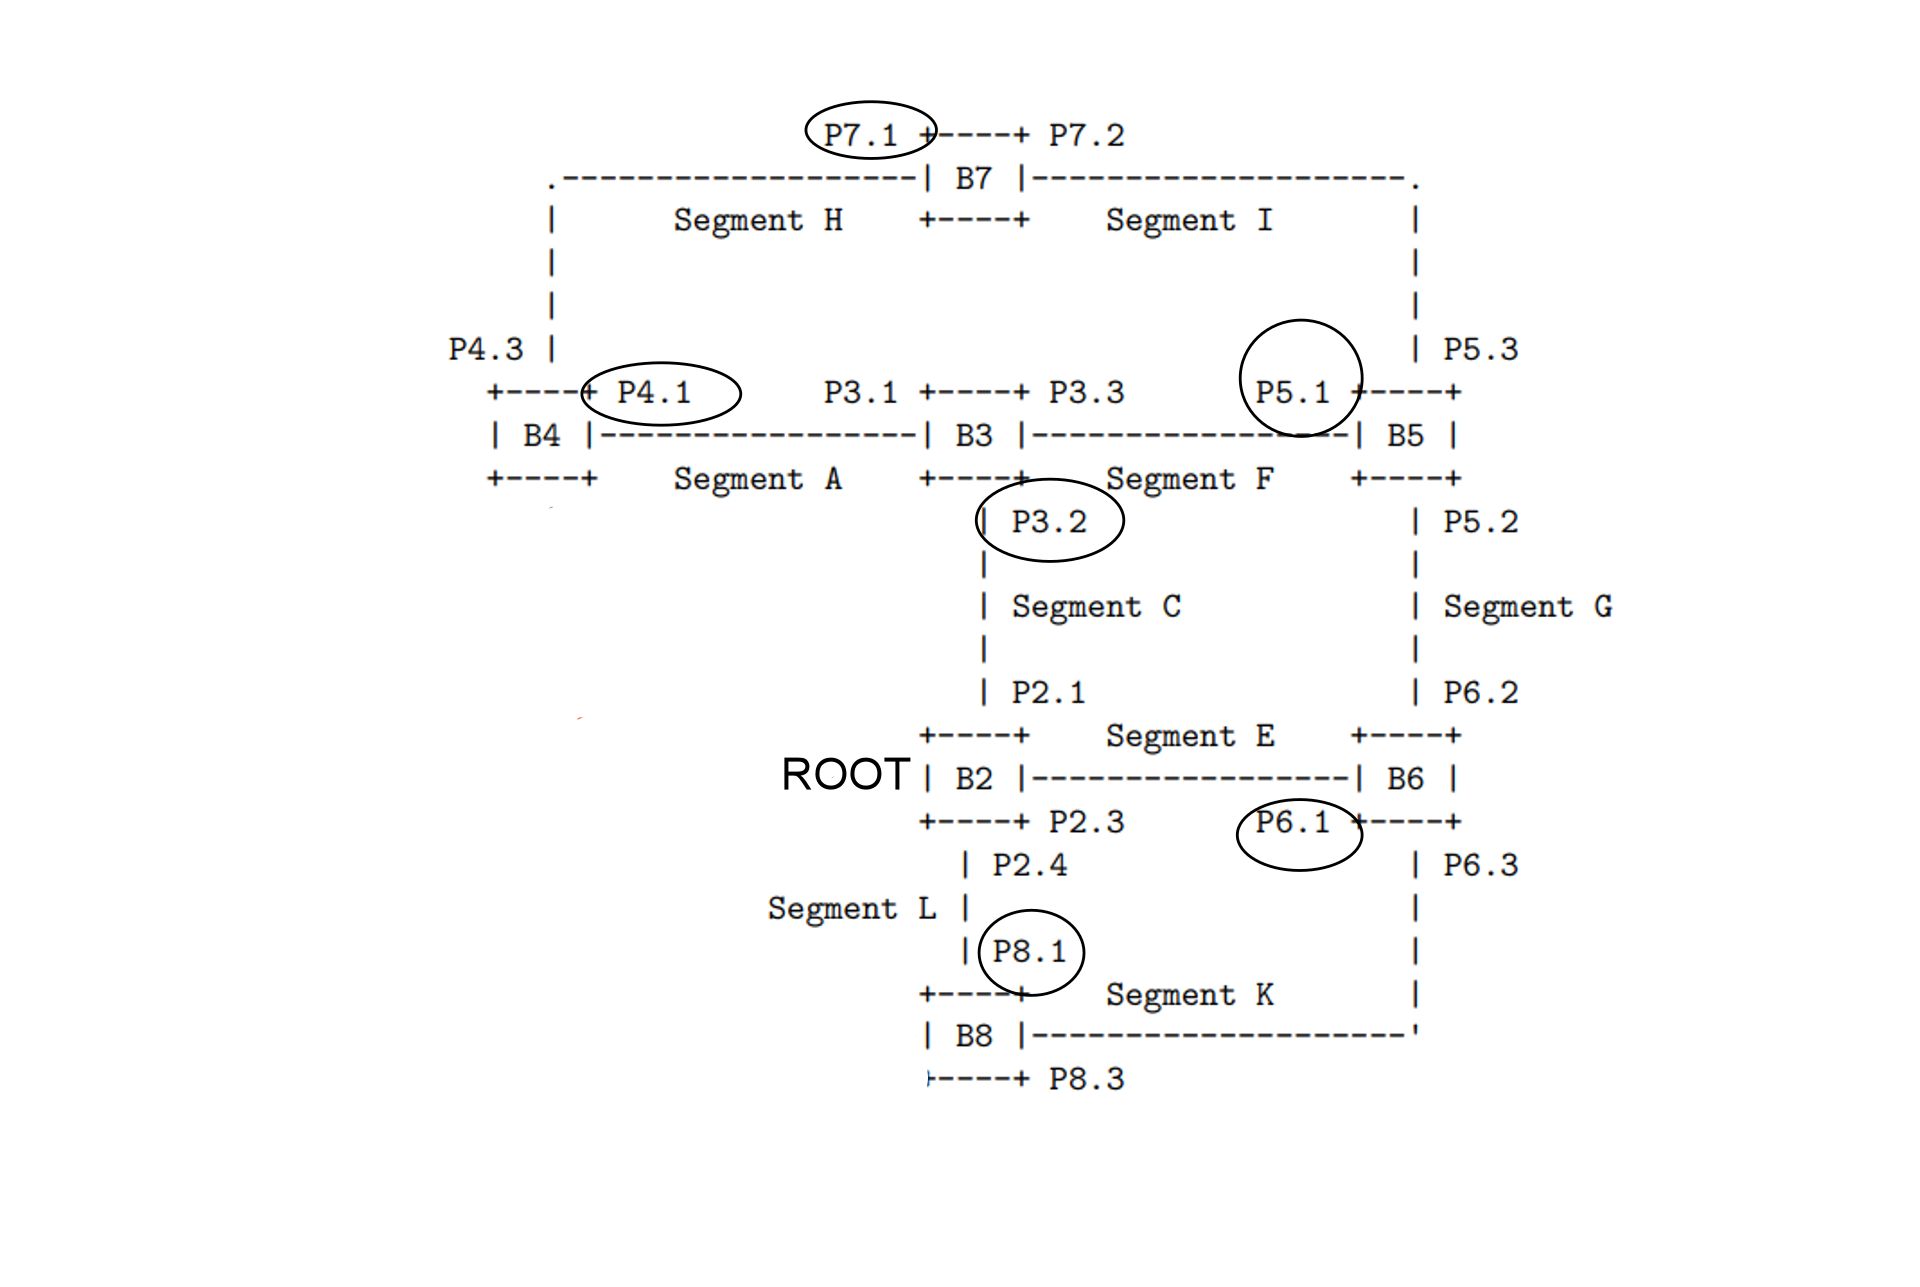
\includegraphics[scale=0.2]{aww-board4.png}\\
ii)
Next we locate designated ports:
First, we selected every port that has root port on the other end of segment.(designated ports in green).\\
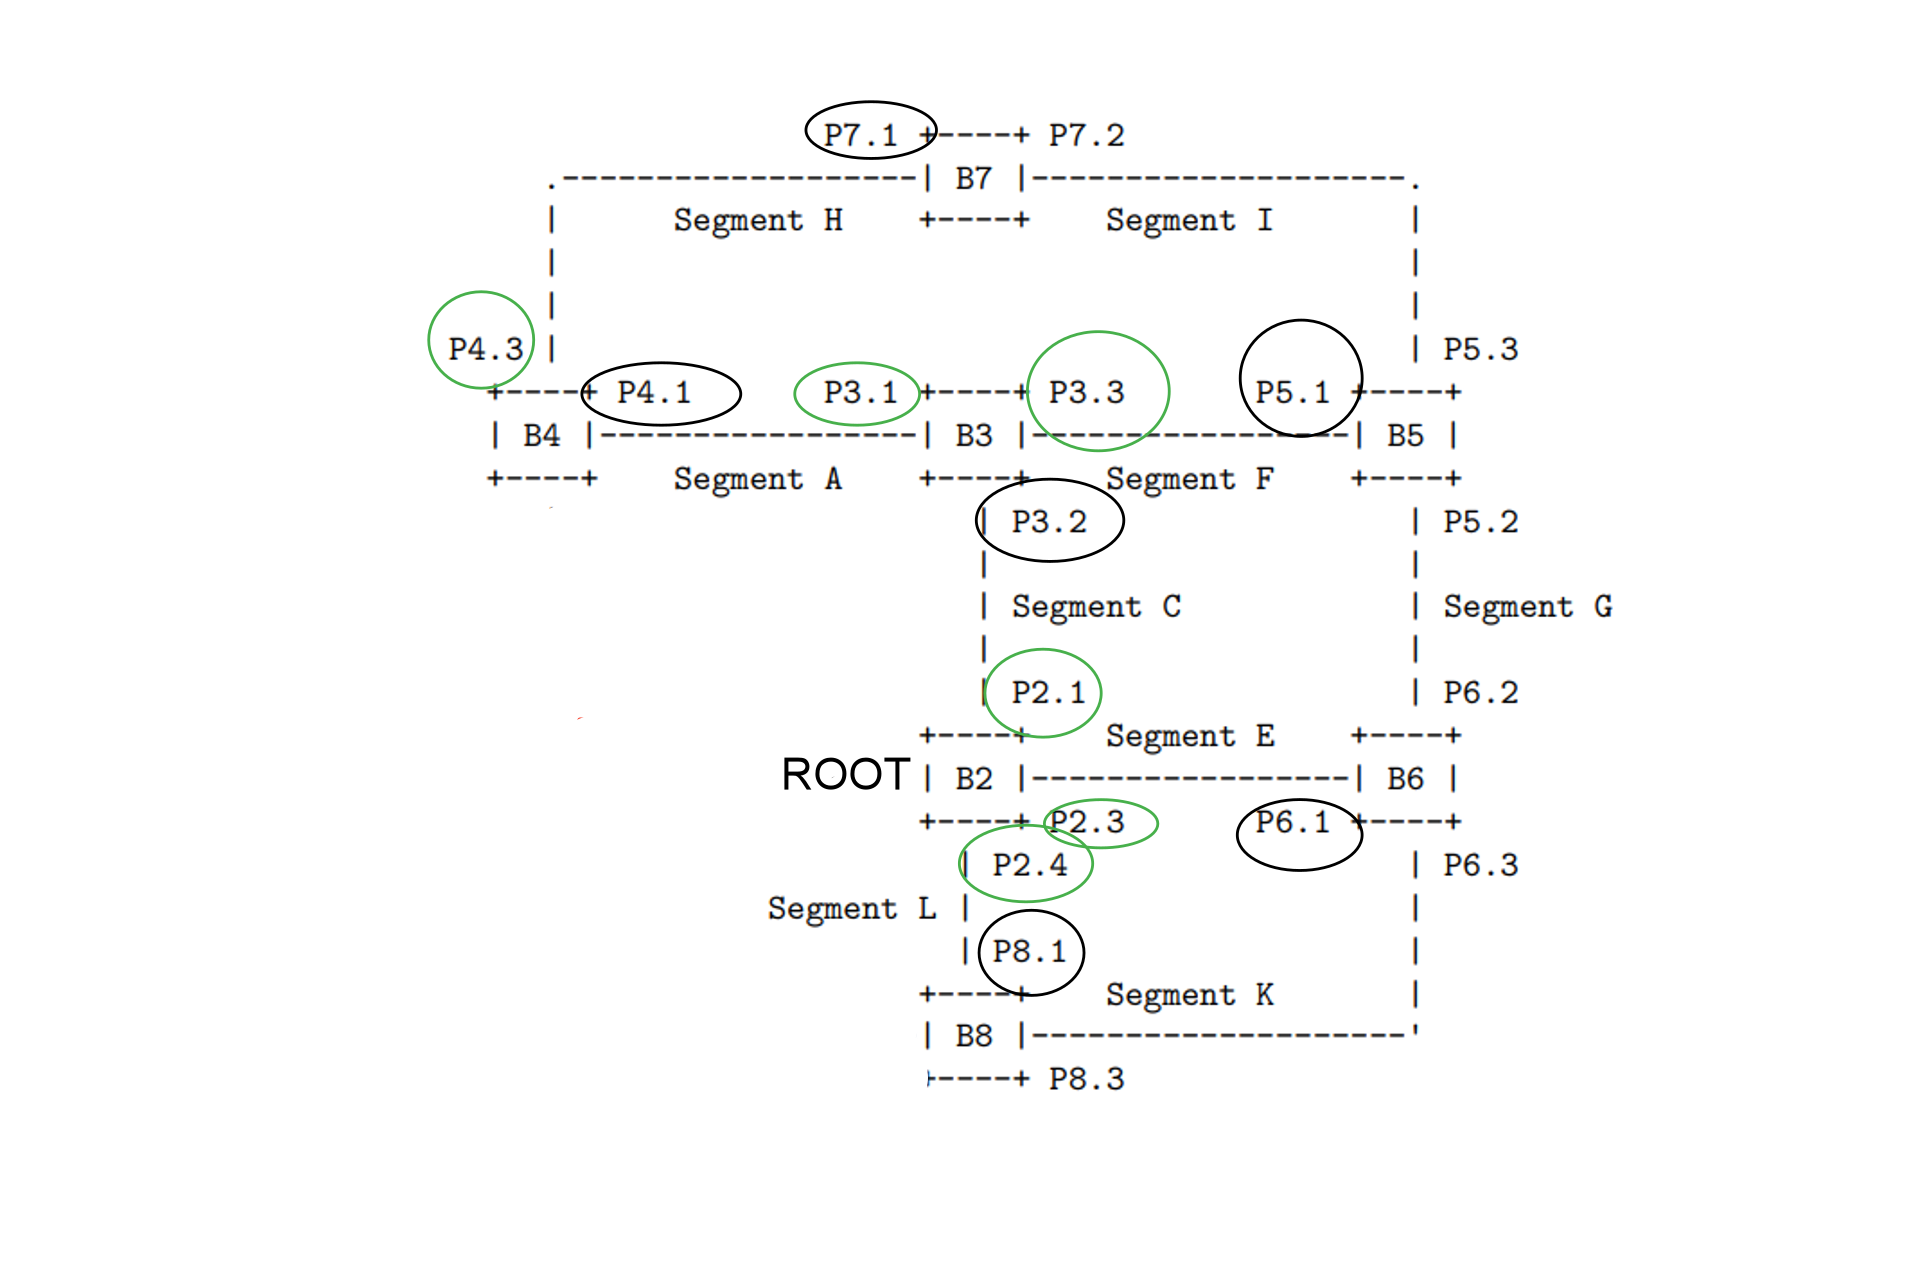
\includegraphics[scale=0.2]{des-port2.png}\\
\\
Next we look on all the unused segments, and select one of the ports on them to be designated port, the other part in next bullet point of answer will be selected as a blocked one.\\
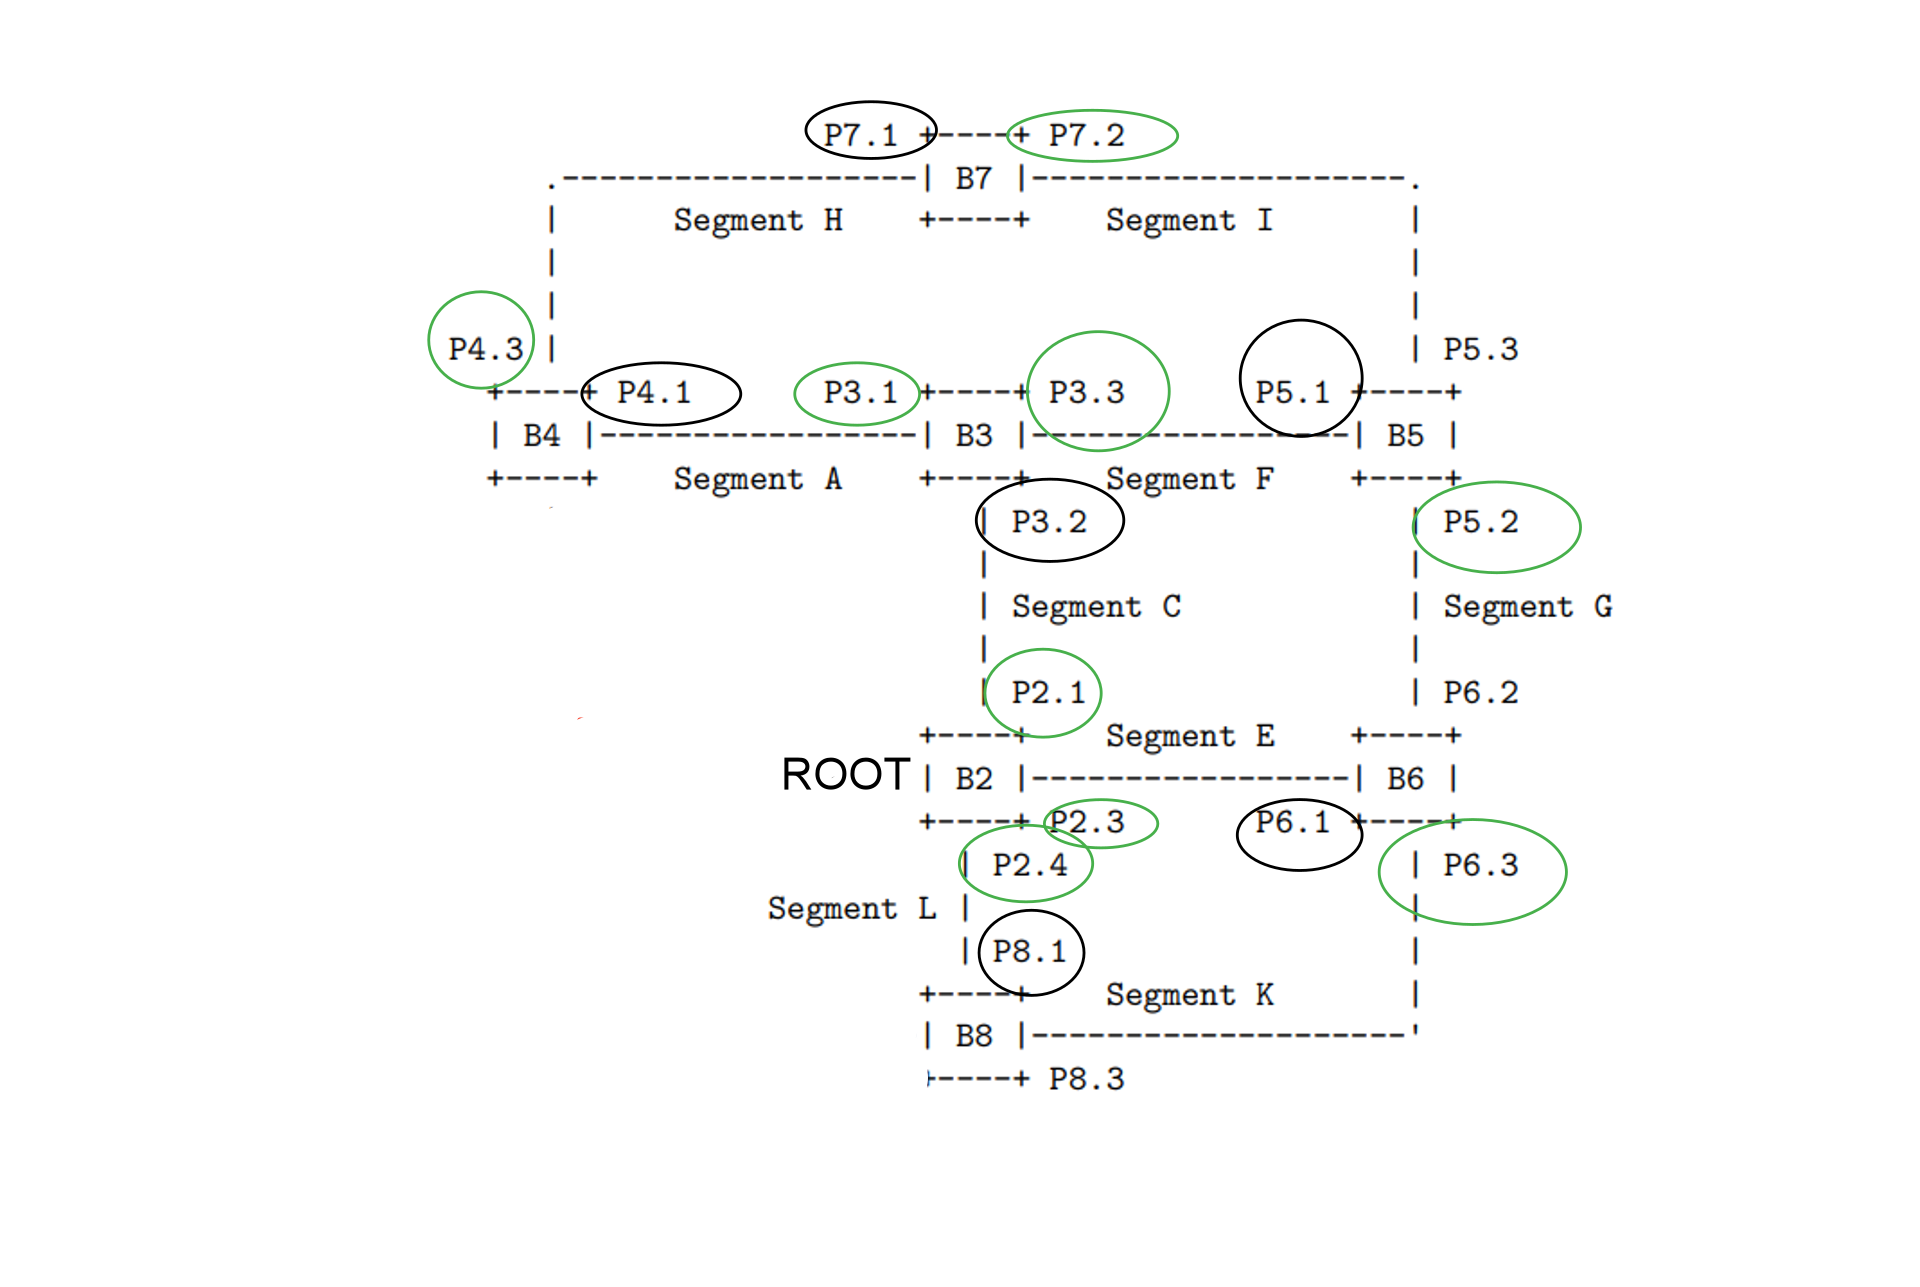
\includegraphics[scale=0.2]{aww-board5.png}
\\\\
iii)All the other ports are blocked ports(circled in red).\\
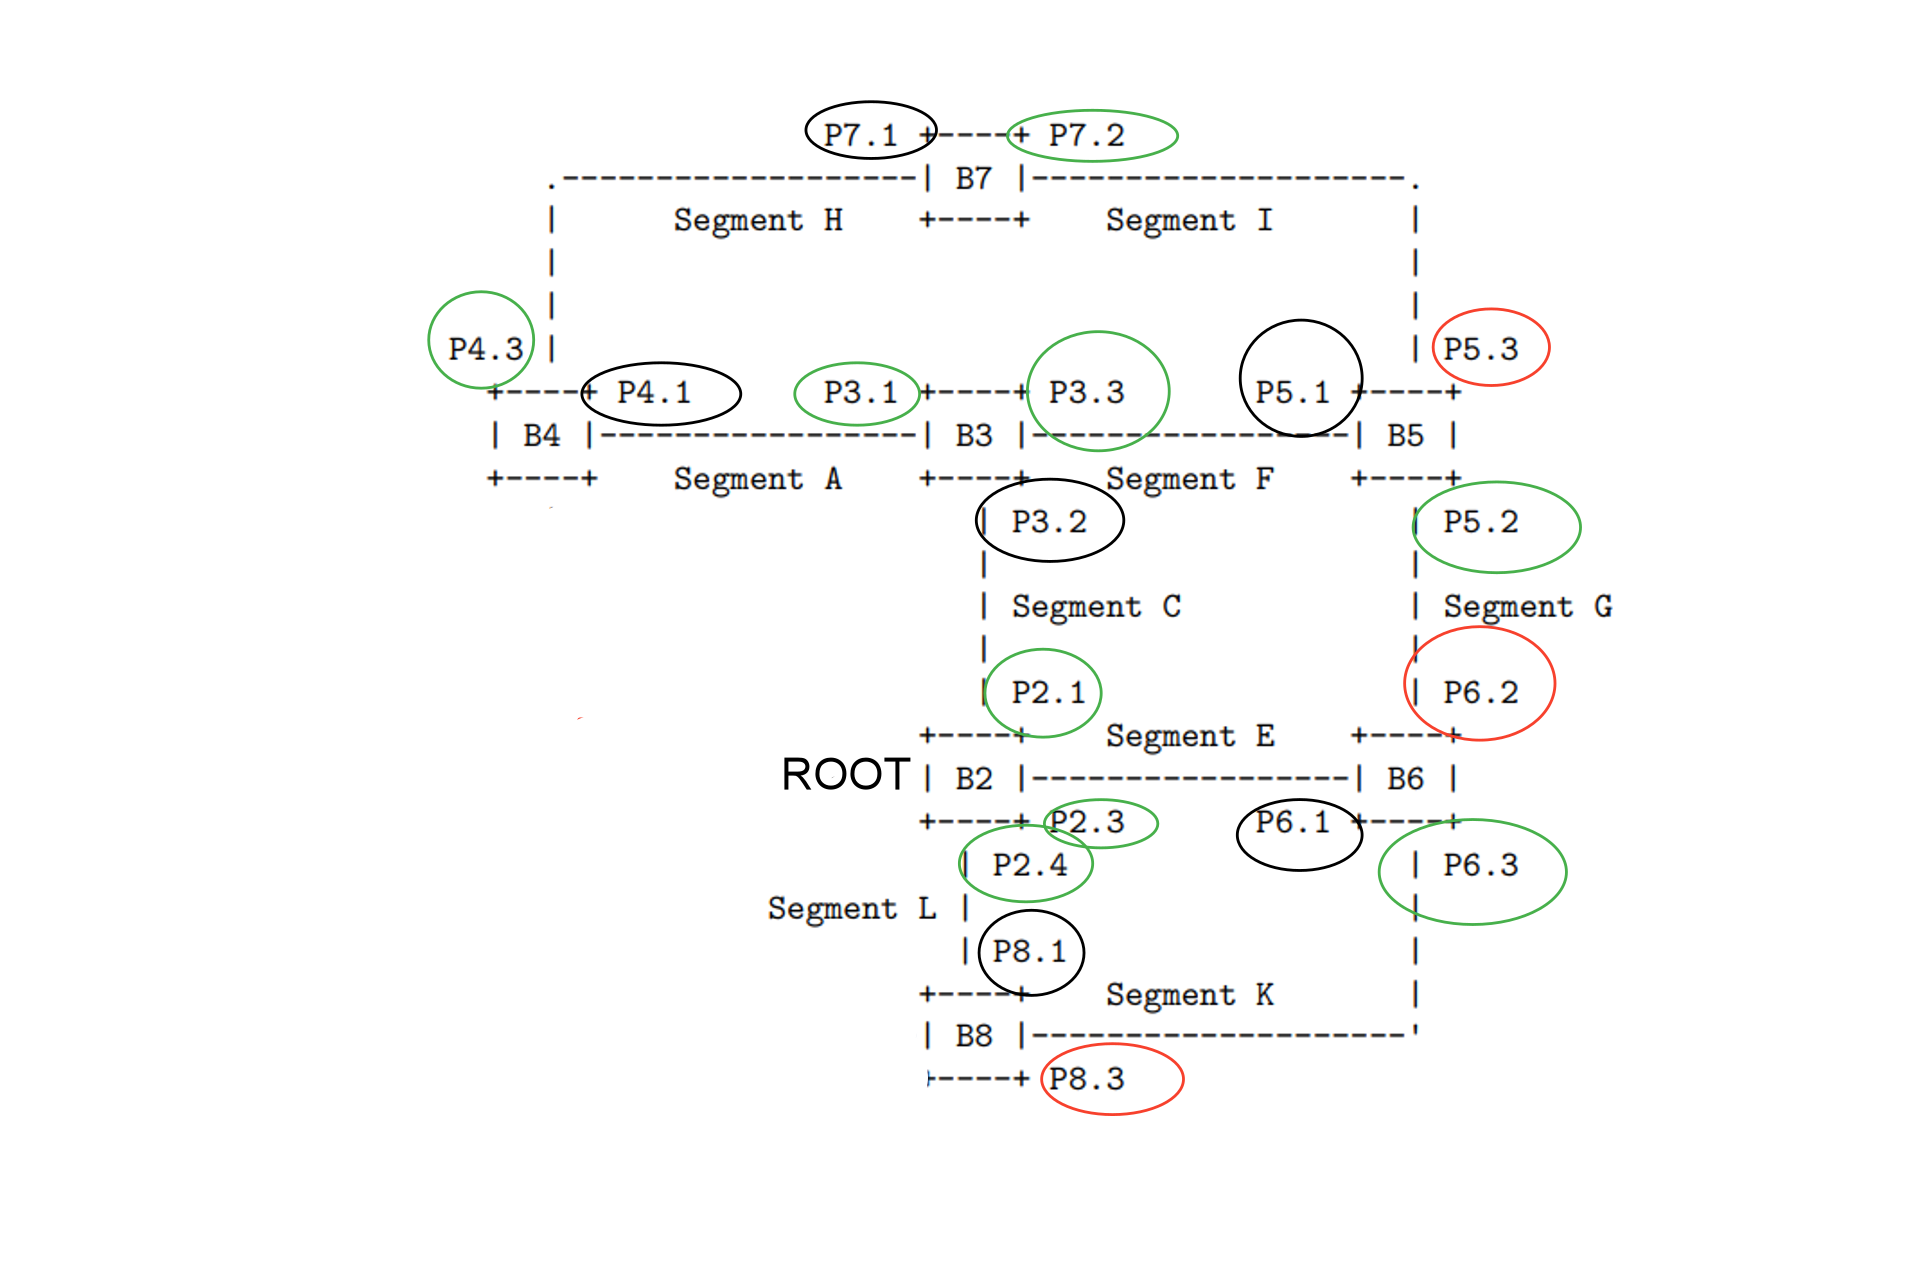
\includegraphics[scale=0.2]{aww-board6.png}\\
\\
\\
\problem{}{0}
\solution
a)\\
According to capture file properties 106280 packets or 19689056 bytes got captured. \\
Ethernet broadcast address is represented by address FF-FF-FF-FF-FF-FF. 52837 packets were transferred, equivalent to 6,826 kb.\\Percentage of broadcast packets is 0.49714. \\Percentage of broadcast bytes is 0.34669005969.\\
b)\\
\begin{verbatim}
The MAC address of the source is Cisco_80:d5:55 or 00:0c:30:89:d5:55.
Destination: Spanning-tree-(for-bridges)_00 (01:80:c2:00:00:00)
The PDUs were sent approximately every 2 seconds.
Root Bridge ID: Cisco_04:33:40 (50:57:a8:04:33:40)
\end{verbatim}
c)\\
Yes, BROWSER, CDP, DTP, IPX RIP, NBIPX, ZIP.\\
\end{document}